
% Este documento LaTeX fue dise�ado por profesores  del Departamento de Matem�ticas 
% de la Universidad de Antioqua (http://ciencias.udea.edu.co/). Usted puede modificarlo
% y personalizarlo a su gusto bajo los t�rminos de la licencia de documentaci�n libre GNU.
% http://es.wikipedia.org/w/index.php?title=Licencia_de_documentaci%C3%B3n_libre_de_GNU&oldid=15717448

%\documentclass[serif,9pt]{beamer}
%\setbeamertemplate{navigation symbols}{}

%\setbeamercolor{frametitle}{fg=black,bg=white}
%\setbeamercolor{title}{fg=black,bg=yellow!85!orange}
%\usetheme{AnnArbor}

%\documentclass{beamer}

\documentclass[serif,9pt]{beamer}
\usetheme{Pittsburgh}
%\usepackage{german}
\usepackage[latin1]{inputenc}




\begin{document}

\title[El trafico automovilistico en las ciudades]{El trafico automovilistico en las ciudades: Un posible sistema complejo}  
\author[Allan Ulises Zepeda Ibarra]{Allan Ulises Zepeda Ibarra}

\date[Junio, 2015]




\begin{frame}
\titlepage
\end{frame}

\begin{frame}\frametitle{�Que es el Trafico?}
Se refiere de manera urbana, a la condici\'on de un flujo vehicular que se ve saturado debido al exceso de demanda de las v\'\i as\\
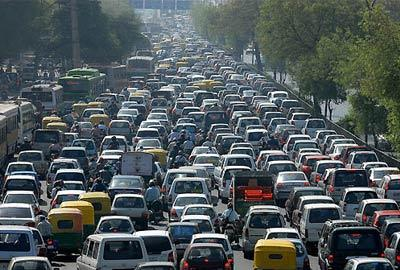
\includegraphics[width=8cm, height=4cm]{1.jpg}
\end{frame} 

\begin{frame}\frametitle{Causas}
La congesti\'on del tr\'afico se produce cuando el volumen del tr\'afico o de la districuci\'on normal del transporte genera una demanda de espacio masyor a la disponible\\
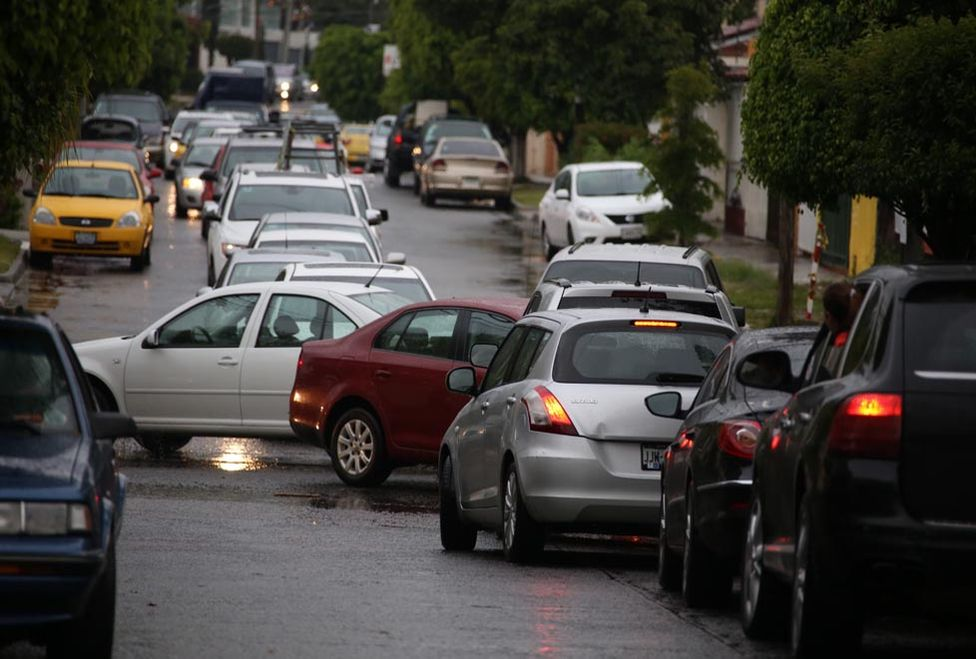
\includegraphics[width=8cm, height=4cm]{2.jpg}
\end{frame} 

\begin{frame}\frametitle{Complejidad}
Elemento primitivo: autom\'ovil\\
Prediccion de comportamiento: No se puede predecir cuando o donde aparecer\'a\\
Adaptativo\\
Comportamiento colectitivo no trivial\\
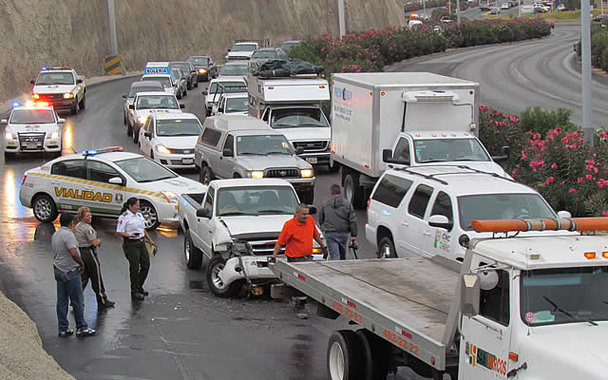
\includegraphics[width=8cm, height=4cm]{3.jpg}
\end{frame} 


\end{document}